\chapter{Orchestrating Transformation Networks 
    \pgsize{20 p.}
}
\label{chap:orchestration}

Problem statement: \todo{Precisely define problem statement}

\todo{Beispiel warum mehrfache Ausführung nötig, warum also manche Infos erst durch andere bx reinkommen, die bei einer bx isoliert nicht relevant sind.}

\todo{Zeigen: ionfluenz führt zu Konvergenz. Aber konfluenz ist zu s arke Anforderung, außerdem heißt Konvergenz, dass egal welche Reihenfolge der Transformationen man wählt am Ende immer das gleiche Ergebnis rauskommt. Das muss aber nicht so sein. Gebe Beispiel mit groß klein Schreibung, wo je nach Reihe folge verschieden elosungen rauskommen}

\todo{Diss: Konvergenz einführen, hinreichende Eigenschaft? Notwendige Eigenschaft?}

\todo{Property for orchestration: if no consistent solution found then there is no further transformation that could be executed without alternation or because no transforamtion is applicable (undefined for current state, e.g. because of monotony)}

\todo{Basically two reasons for not finding consistent solution:
1. relations are contradictory
2. transformations make choices of models that are always incompatible to others}

\todo{Discuss confluence and convergence!}

\section{Restrictions vs. Conservativeness}

\todo{First restriction: Input delta of APP only contains changes to one model -> no synchronisation}
\todo{Second restriction: Input delta is not rejected}
\todo{Third restriction: Generated deltas are monotone}

From a theoretical perspective, it is always possible to a specify consistency relations according to the definition, as it is just a subset of elements.
It is also always possible to define a consistency preservation rule for a consistency relation according to its definition, as can simply return any any element of the relation.
\todo{This is not true: the source model may not be in the relation, then its not possible, at least with the current definition. With a synchronizing transformation, any modification can be made to both models, then its fine.}
The generalization function is generic, so it can always be applied.
Finally, the consistency preservation application function is an artifact that cannot be easily specified according to the definition for a given set of consistency preservation rules.
It is always possible to have a set of consistency preservation rules for which no application function can be defined that returns a consistent result for at least one input model and change tuple, as there is not sequence of consistency preservation rules that achieves that.
\todo{Example!}
Even worse, the problem to define such a function is Turing-complete, which makes it impossible to decide whether such a function exists.
\todo{Show Turing-completeness}
Consequence: From a theoretical perspective, this function is the crucial part!

Essential problem: One transformation may restore consistency between A and B and another between A and C. If then a transformation restores consistency between B and C, the resulting B' and C' may not be consistent A anymore.

Alternative to an app function: Define a \emph{well-definedness} property for a set of transformations, requiring that they can be executed in any order to always terminate consistently. However, this is a very strict requirement, which can usually not be fulfilled, so we do not further investigate that.
\todo{Give simple example why that does not work.}


Best-behaved app function: Whenever there is a sequence of CPRs, the app function finds item. This is still not possible due to Turing-completeness. The function would need to decide whether the network terminates or not.

Only achievable app function is a best-effort (i.e. conservative) function: A function that either returns a consistent set of models or that does return bottom. Not making a statement about how often a correct result is returned in comparison to how often it is possible.

This approach is conservative. The question is then, how high the degree of conservativeness is. In the worst case, a function that always returns bottom would fulfill the definition, but that is not what we want. We want to reduce conservativeness.

Goal: Find a solution in as many cases as possible, abort in the others (conservatively). There are two subgoals to achieve that:
1. Function must be correct, i.e. always terminate (no endless sequence of CPR) and terminate in a consistent state
2. Function must be as less conservative as possible

It is clear that we cannot give a closed function for APP that just by a given change returns a sequence of CPR that results in a consistent state. APP has to be calculated dynamically during execution. Therefore we consider it as an algorithm in the following.

Annahmen:
\begin{itemize}
    \item Nutzeränderungen dürfen nicht rückgängig gemacht werden.
    \item Nutzeränderungen lassen sich so feingranular zerlegen, dass, falls durch die Erzeugung/Änderung eine Konsistenzrelation verletzt wird, es in jeder unabhängigen Teilmenge von Konsistenzrelationen eine verletzte Konsistenzrelation gibt, für die die geänderten Elemente einem Condition Elemente entsprechen, es also insbesondere keine Teilmenge der geänderten Element gibt, die bereits dieses Condition Element sind. Ansonsten ist durch unsere Kompatibilitäts-Definition nicht sichergestellt, dass eine konsistente Modellmenge gefunden werden kann.
\end{itemize}

Annahme an Transformationen:
\begin{itemize}
    \item Muss eine Transformation mit jedem beliebigen Delta umgehen können müssen? Eine Einschränkung auf Monotonie würde dies verhindern. Bzw. wir müssten zeigen, dass es Konsistenzrelationen gibt, die unter der Anforderung an Monotonie nicht wiederhergestellt werden können. Bspw. fügt eine andere Transformation 3 Elemente hinzu, wo zwei mit dem anderen entsprechend der Konsistenzrelationen korrelieren und somit keine Witness-Struktur aufgebaut werden kann, die Konsistenz beweist. Das lässt sich durch Hinzufügen weiterer Elemente potentiell nicht auflösen (siehe Beispiele im SoSym-Paper).
\end{itemize}


\section{Considerations}

Zu diskutierende Dinge:
\begin{itemize}
    \item Im Allgemeinen könnte eine Transformation beliebige dieser Deltasequenzen modifizieren. Wir verlangen jedoch, dass eine Transformation nur Deltas anhängt, also die Sequenzen länger werden
    \item Genauer beschränken wir auch, welche Sequenzen eine Transformation sehen und ändern darf, genau gesagt darf sie die Sequenzen von zwei Modellen sehen und eine davon verlängern.
    \item Hier kommt bereits der Unterschied zu bisherigen Transformationen, denn die sehen nur Deltas an einem Modell und erzeugen Deltas an dem anderen. Das ist bei uns schon gänzlich anders. Bidirektionale Transformationen unterstützen das im Übrigen auch nicht, sondern sind nur Spezifikationen, aus denen sich Wiederherstellungsroutinen für beide Richtungen ableiten lassen (siehe Stevens 2010)
\end{itemize}


Trivialisierung des Problems:
\begin{itemize}
    \item Ohne weitere Annahmen ist das immer dadurch erreichbar, dass die Transformationen einen beliebigen anderen Zustand der Modelle produzieren. Im einfachsten Fall liefert jede Transformation immer die gleichen konsistenten Modelle zurück, unabhängig von der Änderung. Dann ist der Endzustand der Modelle nach der Ausführung des Netzwerks immer der gleiche.
    \item Das ist im allgemeinen aber nicht Fall. Letztendlich trifft jede Transformation lokale Entscheidungen. Beispielsweise könnte jede einzelne Transformation gegeben eine beliebige Änderung immer dieselben Modelle (bzw. Änderungen die dazu führen) zurückliefern (im trivialsten Fall leere Modelle). Dann erfüllt jede Transformation ihre Korrektheitseigenschaft bzgl. ihrer Relation, aber das Netzwerk muss nicht korrekt sein, da bspw. T(A,B) und T(B,C) sich immer für verschiedene Instanzen von B entscheiden. Es gäbe somit nie eine konsistente Lösung für eine beliebige Ausführungsreihenfolge der Transformationen, auch wenn die Relationen das erlauben würden.
    \item Beispiel mit Namen, wo eine Transformation immer den großen Namen zurückliefert, die andere immer den kleinen. T(A,B) bildet A auf gleiches B ab und beide auf kleine Schreibweise, obwohl beide erlaubt sind. Erzeuge A="a", dadurch B="a". T(B,C) bildet B auf C ab und beide auf große Schreibweise, obwohl beide erlaubt sind. Somit macht sie das zu B="A" und C="A". Nun wird T(A,B) wieder beide klein machen usw. Allerdings wäre eine insgesamt valide Lösung einfach alle groß oder alle klein zu machen, aber die Transformationen finden diesen Zustand nicht. 
    \item Allgemeiner ist zu sagen, dass ein Transformationsnetzwerk eine Turing-Maschine emulieren kann. \todo{Nachweisen!}
    Im allgemeinen terminiert das Netzwerk somit nicht, schlimmer noch, es ist unentscheidbar, ob das Netzwerk hält (siehe Halteproblem).
    \item Dies zeigt bereits, dass keine Ausführungsfunktion definiert werden kann, die immer ein konsistentes Ergebnis liefert.
    \item Wir versuchen daher Annahmen an Transformationen zu finden, um diese Fälle auszuschließen bzw. systematisch zu verringern. 
    \item Außerdem möchten wir eine Ausführungsfunktion haben, die ein konsistentes Ergebnis liefert oder einen Fehler, denn es muss nicht immer eine korrekte Lösung geben. Ziel ist es dann die Anzahl der Fälle, in denen sie einen Fehler zurückgibt, zu reduzieren.
\end{itemize}


Zielsetzung:
\begin{itemize}
    \item Korrekte Anwendungsfunktion finden (in bestehenden Arbeiten~\cite{stevens2017a}) auch "Resolution" genannt (formal definieren!):
    \item Welche Anforderungen müssen wir dafür an die Transformationen stellen, damit solch eine Funktion definiert werden kann?
    \item Wir bezeichnen das Transformationsnetzwerk, in dem eine Transformation eingesetzt wird, als "Kontext"
    \item Welche dieser Eigenschaften kann die einzelne Transformation (ohne Kenntnis der anderen) erfüllen und für welche muss der Kontext (d.h. die anderen Transformationen) bekannt sein?
    \item $\Rightarrow$ Interesse an "kontextfreien" Eigenschaften (lassen sich ohne Kenntnis der anderen Transformationen sicherstellen -> Wiederverwendbarkeit) und "kontextsensitiven" Eigenschaften (Erfüllung der Eigenschaft nur durch Kenntnis über das Transformationsnetzwerk möglich)
    \item Kontextfreie Eigenschaften involvieren solche, die wir eh schon von Transformationen kennen (Korrektheit einer Transformation, Hippokratie etc.) und solche, die dadurch zustande kommen, dass man weiß, dass diese Transformation in einem Netzwerk eingesetzt werden soll.
    \item Zielsetzungsoptionen:
    \begin{itemize}
        \item Wir schränken die Transformationen so ein, dass es immer mindestens eine Ausführungsreihenfolge der Transformationen gibt, sodass für jede beliebige Änderung ein konsistentes Ergebnis durch Anwenden der Transformationen gefunden werden kann
        \item Wir akzeptieren, dass es Änderungen gibt, für die das Netzwerk kein konsistentes Ergebnis produzieren kann. Dann muss das Netzwerk (mindestens) in diesen Fällen mit einer Fehlermeldung terminieren.
        \item Eine Option ist, dass das Netzwerk dieses Verhalten nur approximiert bzw. approximieren kann, dann muss es sich konservativ verhalten, d.h. im Fall, dass es keine Lösung gibt, auf jeden Fall eine Fehlermeldung geben, und im Fall, in dem es eine Lösung gibt, diese bestenfalls finden oder ausgeben, dass es keine finden kann (d.h. keine False Positives bzw. Nicht-Terminierung). Ziel ist es dann den Grad der Konservativität zu minimieren.
    \end{itemize}
    \item Lösungsoptionen (Grad der Einschränkung an die Transformationen):
    \begin{itemize}
        \item Hohe Einschränkung: Jede beliebige Reihenfolge von ausgeführten Transformationen führt letztendlich zu einem korrekten Ergebnis (Fixpunktiteration -- Allquantifizierung) -- Hippokratie-Eigenschaft sorgt dafür, dass keine Transformation wieder etwas ändert, wenn Konsistenz bereits hergestellt ist.
        Diese Eigenschaft ist in der Praxis möglicherweise zu strikt, da sie sehr starke Anforderungen an die Transformationen stellen müsste. Dafür wäre aber die Anwendungsfunktion trivial.
        \item Mittlere Einschränkung: Es gibt eine Reihenfolge von ausgeführten Transformationen für jede Änderung die terminiert (Existenzquantifizierung) und die Ausführungsfunktion findet diese Reihenfolge.
        Utopisch, dass die Anwendungsfunktion aus (potentiell sehr mächtigen) Transformationen die richtige Reihenfolge errechnen kann. Dafür aber (möglicherweise) weniger Anforderungen an die Transformationen (zumindest nicht mehr Anforderungen, denn die Allquantifzierung induziert die Existenzquantifizierung). Eine Funktion könnte dann zumindest nach best-effort versuchen, die richtige Reihenfolge zu finden und konservativ abbrechen, wenn sie diese nicht finden kann (also entweder konsistent terminieren oder terminieren mit der Aussage, dass es entweder keine solche Reihenfolge gibt -- bei relaxierten Anforderungen -- oder dass es sie nicht finden kann).  
        \item Geringe Einschränkung: Es gibt potentiell keine Reihenfolge der Transformationen, die bei einer Änderung zu einer konsistenten Lösung kommt. Hier müsste die Ausführungsfunktion entsprechend einen Fehler ausgeben.
        \item Bestehende Arbeiten (\cite{stevens2017a}) schlagen auch vor eine Baumstruktur zu berechnen (Spannbaum), in dem nur entlang der Baumkanten die Transformationen ausgeführt werden. Dies ist jedoch eine starke Einschränkung daran, was die Transformationen ausdrücken können. Betrachtet man beispielsweise PCM, UML und Java, und hat eine Änderung in PCM. Dann könnte der Spannbaum entweder PCM -> UML -> Java sein, oder PCM -> UML + PCM -> Java. In ersterem Fall würde Verhaltensbeschreibung, die von PCM nach Java übertragen, aber in UML nicht dargestellt wird, nicht übertragen. Im zweiten Fall würde zusätzliche Information zwischen UML und Java nicht propagiert (Beispiel?) --> Hier sollte auf das Properties-Kapitel verwiesen werden, wo diese "Bottlenecks" erklärt sein sollten, inklusive einem Beispiel, die allgemein Baumstrukturen für Transformationsnetwerke ausschließen.
    \end{itemize}
    \item Dies setzt voraus, dass die Transformationen und die Anwendungsfunktion mit jeder beliebigen Nutzer-Änderung umgehen kann. Man kann jedoch auch verlangen, dass die Anwendungsfunktion genau dann, wenn es überhaupt eine Ausführungsreihenfolge gibt, diese findet, und sonst einen Fehler ausgibt.
    \item \textbf{Wichtig:} Im Allgemeinen kann eine Ausführungsfunktion keine terminierende Reihenfolge berechnen, da die Transformationen Turing-vollständig sind und deshalb die Frage, welche Reihenfolge zu einer Terminierung führt, unentscheidbar ist (Halteproblem). Daher können wir nur einen konservativen Algorithmus angeben, der ein sinnvolles Abbruchkriterium definiert, mit dem die Ausführung beendet wird, auch wenn potentiell eine Lösung hätte gefunden werden können. Die Fragestellung ist also, wie die Ausführungsfunktion aussehen muss, damit sie in möglichst vielen Fällen, in denen es eine terminierenden Reihenfolge gibt, diese auch findet. Insbesondere lässt sich somit keine geschlossene Form für die Ausführungsfunktion angeben, sondern nur ein Algorithmus, der zur Laufzeit eine Reihenfolge (dynamisch) festlegt.
\end{itemize}


Problemraum:
\begin{itemize}
    \item Ziel ist, dass ein Netzwerk von Transformationen nach einer Änderung in einem konsistenten Zustand terminiert. D.h. Korrektheit stellt Anforderungen an \emph{Terminierung}, sowie den \emph{Zustand} bei Terminierung.
    \item Folgende Abweichungen davon können auftreten:
    \begin{enumerate}
        \item Nicht-Terminierung: Das Netzwerk terminiert nicht. Das bedeutet im Prinzip, dass die Ausführungsfunktion (bzw. der Laufzeit-Algorithmus, der die Funktion dynamisch emuliert) nicht \emph{sound} ist. Soundness der Ausführungsfunktion setzt voraus, dass die berechnet Aufrufsequenz endlich ist. Wenn die Ausführung nicht terminiert, bedeutet das, dass entweder die gleichen Zustände mehrfach durchlaufen werden oder eine Sequenz unendlich vieler Zustände produziert wird. Denn wenn beides nicht der Fall ist, gibt es eine endliche Sequenz unterschiedlicher Zustände, d.h. Terminierung. Das bedeutet, dass es folgende zwei Möglichkeiten gibt:
        \begin{itemize}
            \item Alternierung: Die gleichen Zustände werden mehrfach durchlaufen.
            \item Divergenz: Es werden unendlich viele Zustände produziert.
        \end{itemize}
        \item Inkonsistente Terminierung: Die Ausführungsfunktion bzw. der Algorithmus beendet die Ausführung, aber in einem inkonsistenten Zustand. Hier lassen sich ebenfalls wieder zwei Fälle unterscheiden.
        \begin{itemize}
            \item Unerkannte Inkonsistenz: Der Algorithmus terminiert und denkt, der Zielzustand wäre konsistent. Dies bedeutet aber direkt, dass nicht alle Konsistenzrelationen erfüllt sind, was, zumindest in der Theorie, einfach zu prüfen wäre (entweder durch Prüfung der Relationen oder durch Ausführung der hippokratischen Transformationen, die alle nichts tun dürften)
            \item Erkannte Inkonsistenz: Der Algorithmus terminiert, wissend dass die Lösung nicht konsistent ist. Dies kann entweder sein, weil eine Transformation für zwei Modelle in einem inkonsistenten Zustand nicht mehr anwendbar ist, oder weil irgendein anderes Abbruchkriterium erreicht ist.
        \end{itemize}
    \end{enumerate}
\end{itemize}


Notwendigkeit Transformationen oder Anwendungsfunktion einzuschränken:
\begin{itemize}
    \item Zeigen, dass es Beispiele gibt, in denen es keine einzige Ausführungsreihenfolge gibt (All-Quantifizierung), die zu einem konsistenten Ergebnis führt:
    \item Zeigen, dass es Beispiele gibt, in denen es unabhängig von der Ausführungsreihenfolge immer zu einer Alternierung kommt
    \item Zeigen, dass es Beispiele gibt, in denen es unabhängig von der Ausführungsreihenfolge immer zu einer Divergenz kommt.
    \item Die Beispiele sollten zeigen, dass wir keine Einschränkungen an die Transformationen machen können, was das Problem aushebelt. D.h. egal welche Einschränkungen ich an die Transformationen definiere, es lassen sich immer Beispiele konstruieren, in denen es keine Ausführungsreihenfolge gibt, in denen sie terminieren.
    \item Mathematisch zeigen, dass Alternierung und Divergenz die einzigen Probleme sind. D.h. wenn nicht der gleiche Zustand mehrmals durchlaufen wird (Alternierung) und es nicht unendlich viele Zustände gibt (Divergenz), dann ist die Folge endlich.
    \item Außerdem mathematisch die Abbildung von Transformationen auf Turing-Maschinen zeigen und damit ableiten, dass allgemeine Netzwerke erstmal nicht terminieren müssen (Abbildung auf Halteproblem)
\end{itemize}

Zielsetzung die Zweite:
\begin{itemize}
    \item Wir definieren möglichst minimale Beschränkungen, die dazu führen, dass das Netzwerk terminiert. D.h. es terminiert entweder konsistent oder es terminiert mit einem Fehler, der sagt, dass entweder keine Konsistenz hergestellt werden kann (es gibt keine Ausführungsreihenfolge der Transformationen, die zu Konsistenz führt) oder dass die Anwendungsfunktion nicht in der Lage war eine passende Ausführungsreihenfolge zu finden (Konservativität)
    \item Zwei Arten von Beschränkungen
    \begin{itemize}
        \item Beschränkungen an die Transformationen, die dazu führen, dass es in mehr Fällen mindestens eine Ausführungsreihenfolge gibt, in der das Netzwerk konsistent terminiert
        \item Beschränkungen an die Ausführungsfunktion, sodass die Ausführung auf jeden Fall terminiert, wenn auch konservativ, d.h. mit Fehler, obwohl es eine korrekte Lösung gegeben hätte.
    \end{itemize}
\end{itemize}



Exkurs: Menge (konsistenter) Modelle bildet keinen topologischen Raum
\begin{itemize}
    \item Topologischer Raum besteht aus Grundmenge und Mengensystem von Teilmengen mit den Eigenschaften, dass die Grundmenge offen ist, der Schnitt endlich vieler Mengen offen und die Vereinigung beliebig vieler Mengen offen ist. 
    \item Die Grundmenge wäre die Menge aller Modellelemente
    \item Diese Menge ist normalweise offen, da z.B. für ein Element mit einem String-Attributwert immer noch das Element mit dem gleichen String-Attributwert plus einem weiteren Symbol in der Menge liegt (und man die Ordnung in der Menge entsprechend definiert). Dass ein Metamodell möglicherweise Einschränkungen definiert und dann im schlimmsten Fall nur ein einziges Modell valide ist, lassen wir hier außen vor.
    \item Betrachten wir nun eine Topologie auf dieser Menge, also ein Mengensystem aus konsistenten Modellen. Leider ist jedoch der Schnitt zweier konsistenter Modelle nicht zwangsläufig konsistent. Insbesondere sind diese Mengen auch nicht offen, da sie die abgeschlossene Menge darstellen, die genau ein Modell beschreiben. 
    \item Somit lässt sich die Definition von Topologien hier nicht anwenden.
\end{itemize}



\section{No Execution Order with Consistent Result}

It is obvious that we can define consistency preservation rules for which the orchestration function cannot find an execution order that returns a consistent tuple of models after certain changes. Consider the example in \autoref{fig:formal:noexecutionorder}. There exists no execution order for any input value that terminates. The transformations will always increase the value, although the defined relations could be fulfilled for the input value, but the transformations never find that solution.

\begin{figure}
    \centering
    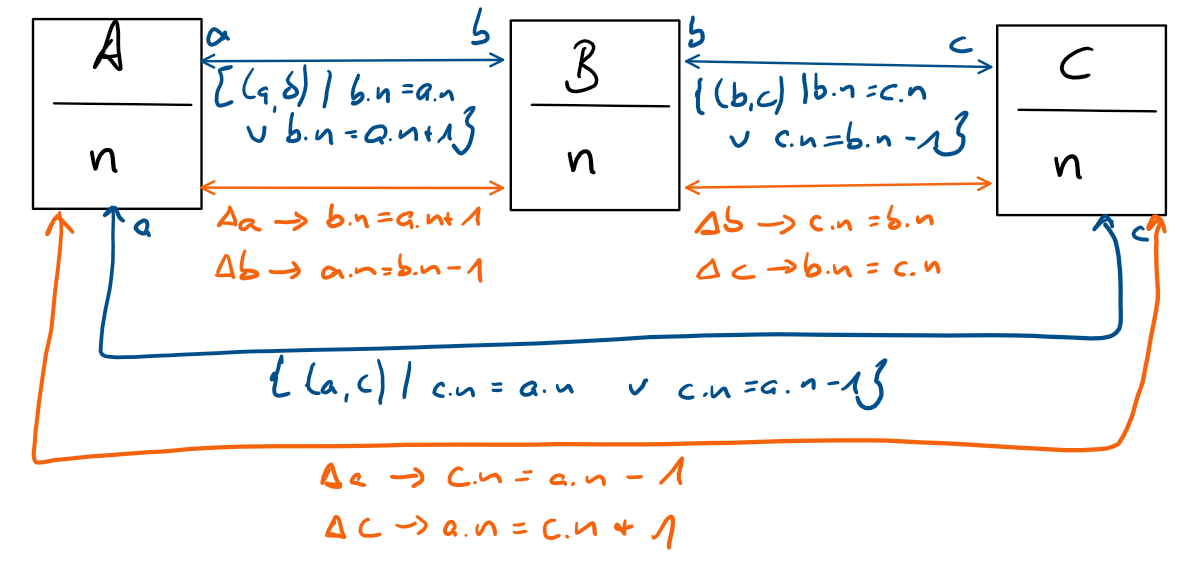
\includegraphics[width=\textwidth]{figures/correctness/formal/divergence_example.png}
    \caption{Example for divergence}
    \label{fig:formal:noexecutionorder}
\end{figure}

Although we will discuss restrictions to relations and transformations that reduce the chance that no solution can be found, it will not be possible to ensure that such a solution can always be found. This is due to the reason that transformations can perform arbitrary changes given that transformations are Turing complete, which should not be restricted, because it is unclear which restrictions could be made without forbidding scenarios that should actually we supported. Thus, we assume that transformations are Turing complete.

We explicitly allow the orchestration function to return a sequence that will, if applied to models and changes to them, not deliver a consistent tuple of models. As discusses, this is supposed to reflect cases in which no such sequence can be calculated.
However, it may be useful to have some notion of \emph{optimality} that ensures that if a sequence that delivers a consistent result exists, the orchestration function is supposed to find it.
Formally, this notion looks as follows.

\begin{definition}[Optimal Consistency Preservation Orchestration Function]
    \todo{Needs to be adapted to transformations rather than CPRs}
    Let $\consistencypreservationruleset{}$ be a set of consistency preservation rules for a set of consistency relations $\consistencyrelationset{CR}$ on metamodels $\metamodeltuple{M} = \tupled{\metamodelsequence{M}{n}}$.
    We say that an orchestration function $\orcfunction{\consistencypreservationruleset{}}$ for these rules is \emph{optimal} if it always returns a sequence that delivers a consistent set of models if possible, i.e.,
    \begin{align*}
        &
        \forall \modeltuple{m} \in \metamodeltupleinstanceset{M} : \forall \changetuple{\metamodeltuple{M}} = \tupled{\change{\metamodel{M}{1}}, \dots, \change{\metamodel{M}{n}}} \in \changeuniverse{\metamodeltuple{M}} :
        \modeltuple{m} \consistenttomath \consistencyrelationset{CR} \Rightarrow \\
        & \formulaskip
        \bigl[ \bigl(
            \exists \consistencypreservationrule{1}, \dots, \consistencypreservationrule{m} \in \consistencypreservationruleset{} : 
            \exists \changetuple{\metamodeltuple{M}}' = \tupled{\change{\metamodel{M}{1}}', \dots, \change{\metamodel{M}{n}}'} \in \changeuniverse{\metamodeltuple{M}} :\\
            & \formulaskip \formulaskip
            \generalizationfunction{\consistencypreservationrule{1}} \concatfunction \dots \concatfunction \generalizationfunction{\consistencypreservationrule{m}}(\modeltuple{m}, \changetuple{\metamodeltuple{M}}) = (\modeltuple{m}, \changetuple{\metamodeltuple{M}}')\\
            & \formulaskip \formulaskip
            \land \tupled{\change{\metamodel{M}{1}}'(\model{m}{1}), \dots, \change{\metamodel{M}{n}}'(\model{m}{n})} \consistenttomath \consistencyrelationset{CR} \bigr) \\
            & \formulaskip
            \Rightarrow \bigl(        
            \exists \consistencypreservationrule{1}', \dots, \consistencypreservationrule{m}' \in \consistencypreservationruleset{} : 
            \exists \changetuple{\metamodeltuple{M}}'' = \tupled{\change{\metamodel{M}{1}}'', \dots, \change{\metamodel{M}{n}}''} \in \changeuniverse{\metamodeltuple{M}} :\\
            & \formulaskip \formulaskip
            \orcfunction{\consistencypreservationruleset{}}(\modeltuple{m}, \changetuple{\metamodeltuple{M}}) = \tupled{\consistencypreservationrule{1}', \dots, \consistencypreservationrule{m}'} \\
            & \formulaskip \formulaskip
            \land \generalizationfunction{\consistencypreservationrule{1}'} \concatfunction \dots \concatfunction \generalizationfunction{\consistencypreservationrule{m}'}(\modeltuple{m}, \changetuple{\metamodeltuple{M}}) = (\modeltuple{m}, \changetuple{\metamodeltuple{M}}'')\\
            & \formulaskip \formulaskip
            \land \tupled{\change{\metamodel{M}{1}}''(\model{m}{1}), \dots, \change{\metamodel{M}{n}}''(\model{m}{n})} \consistenttomath \consistencyrelationset{CR}
        \bigr) \bigr]
    \end{align*}
\end{definition}

Unfortunately, optimality is a property that we cannot request from an orchestration function. Optimality would mean that the orchestration function can decide whether there is sequence of transformations that leads to consistent models and thus terminate.
Due to Turing-completeness of the network this would mean that the orchestration function can decide whether a Turing machine halts, which is proven impossible.
Thus, our only goal can be to achieve optimality as far as possible in terms of reducing the degree of conservativeness, i.e., reduce the cases in which no sequence is found although it exists.

We can define a measure for the optimality of an orchestration function:
\begin{align*}
    &
    Optimality_{\orcfunction{\consistencypreservationruleset{}}} = \frac{\mathtext{\# of model / delta pairs for which the function finds an order that terminate consistently}}{\mathtext{\# of model / delta pairs for which an order that terminates consistently exists}}
\end{align*}

In fact, both these numbers usually infinite, an there is an infinite number of possible models and deltas. However, it does finally not matter for us what the actually value is, but only how to improve that value.
\todo{We have to map that value to compatibility, which reduces the number of potential false orders.}



\subsection{Achieving an Always Correct Application Function}
% This discusses the case that the application function is optimal
\todo{These problem cannot occur if a function fulfills the definition, because it always finds a sequence. So the question is how to fulfill the definition.}

It is easy to achieve that the APP function only terminates in a consistent state, because knowing the relations allows to check whether all relations are fulfilled. 
\todo{Need to define that a transformation may not be able to process a specific change? Then there could be inconsistent terminiation because a transformation cannot be executed anymore.}

Problems due to which the function does not terminate: Alternation and Divergence

Alternation: Run through same state twice
Divergence: Always produce new states without reaching a consistent state

Two possibilities to avoid problems:
1. Make assumptions to transformations that avoid them
2. Detect them dynamically and abort


\subsubsection{Avoiding Alternation / Divergence}

Making assumptions that avoid them is rather hard, as we will show in the following.

\paragraph{Idea:} Require monotony to avoid alternation

We would have to relax the definition of transformation to be monotone, because if a transformation is monotone, it may only append information, but this is not always possible, as can be seen in the following example. A monotone transformation must be able to return bottom if it cannot make further changes to restore consistency to the relation.

\begin{definition}[Monotone Transformation]
    Transformation gets models M and deltas D and produces new deltas D'. Taking the union of the original models M and the new models D'(M), then D(M) must be a subset of that, because other elements would have been added and removed afterwards or elements would have been changes once by D and again in a different way by D'.

    Generally, monotony could also mean that only the same complete model state is not passed twice. \todo{Why dont we do that?}
\end{definition}

This would mean that each transformation only appends changes, i.e., if an element was added/removed, the transformation may not do the inverse. The same applies to attribute/reference changes: if an attribute/reference was already changes it may not be changed again.
This way, it is by design impossible to pass through the same state again. Actually, if a monotone transformation returns bottom, the network has to terminate with a failure.
However, this is hard restriction to transformations. It leads to the fact that in some networks that actually have a simple solution no solution is found at all. This can be easily seen at the example in \autoref{fig:formal:monotonycounterexample}. In the example adding "aa" to the left model, any execution order of the transformations leads to the situation that a previous change must be revoked to result in a consistent state. However, it is possible to derive a consistent state for that input change.

\begin{figure}
    \centering
    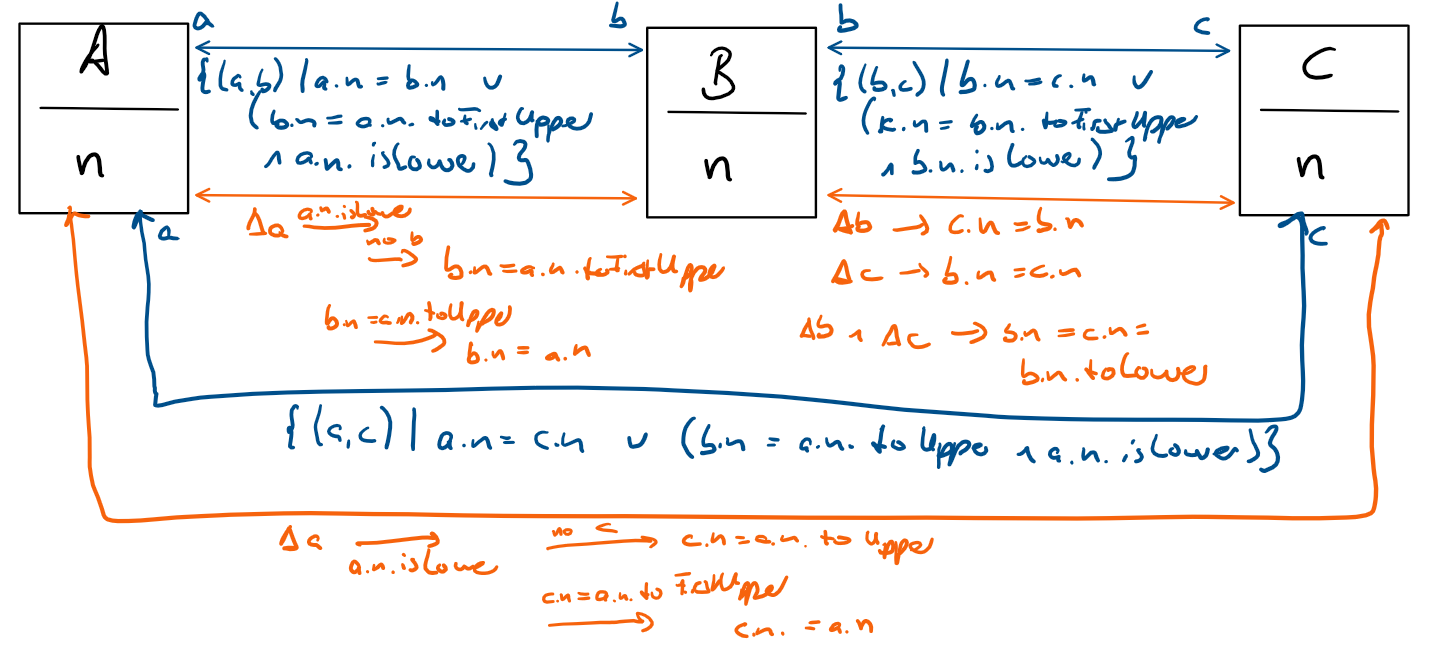
\includegraphics[width=\textwidth]{figures/correctness/formal/monotony_counterexample.png}
    \caption{Counterexample for monotony}
    \label{fig:formal:monotonycounterexample}
\end{figure}

One could now argue that there are binary relations in the example, which may never be fulfilled at all. We will later discuss how far relations that cannot be fulfilled should be restricted. However, in general, this is wanted behavior, because in general it may be necessary that transformations produce intermediate states that are not yet consistent with each other. Otherwise this would means that each transformation is always able to directly deliver a state that is consistent to all other relations, which is especially not possible, because other transformations may add further information to the models. More precisely, a relation may consider <a model consistent to all other models that contain any additional information not affected by the transformation. For example, a UML class model may be considered consistent to all Java models with any implementation of the specified methods, thus to an infinite number of models. Now saying that it should not be allowed that the transformation selects one with an empty implementation because that is not consistent to another relations induced by another transformation, such as the relationship to a component model, does not make any sense. Thus having those relation elements that may be considered locally consistent but will never occur in a globally consistent tuple of models does not make sense.
In the example, we can see that such an inconsistent intermediate state is passed through and afterwards a consistent tuple of models is reached if not requiring monotony.
In consequence, requiring monotony from transformations is a too strict requirement, because it is necessary to run through states that may be changed later on.

\begin{theorem}
    An application function for monotone transformations either returns a consistent model or produce a sequence of CPRs returning delta that return models of always growing size (i.e. it diverges).
\end{theorem}


\paragraph{Divergence cannot be avoided}

There are rather equal network, one that terminates after a long time and one that never terminates. 
Consider the example. The relations are defined in a way such that for any allocation for any of them a consistent tuple of models can be found. However, the transformations are not able to find it because they make "bad" choices from a set of choices that are conflicting. 
This can be seen in the example in \autoref{fig:formal:divergenceexample}.

\begin{figure}
    \centering
    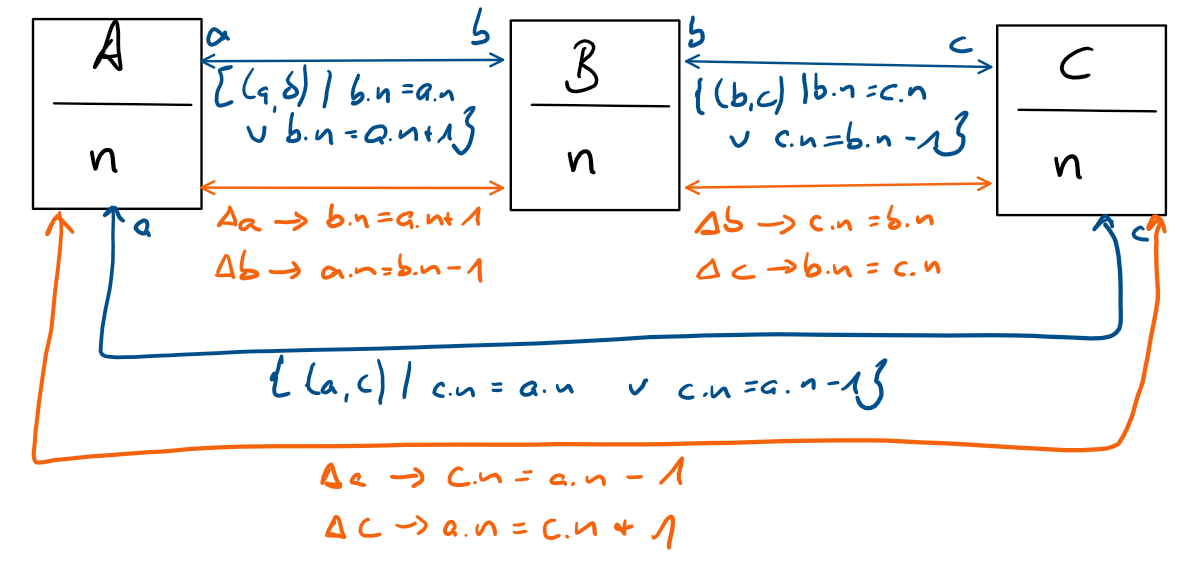
\includegraphics[width=\textwidth]{figures/correctness/formal/divergence_example.png}
    \caption{Example for divergence}
    \label{fig:formal:divergenceexample}
\end{figure}

Thus, systematically avoiding divergence is not possible. 



\paragraph{Detecting Alternation / Divergence}

In consequence, we propose to dynamically deal with alternation / divergence.
To detect alternations, the execution can simply track if a state way already processed. Apart from spatial problems, this does always work.
Finding divergence is not that easy, because it is generally not possible to define an upper bound for the number of executions of a single transformation.
This is due to the reason that, again, this conflicts with the Halting problem.
We can see this at the simple example in \autoref{fig:formal:noupperboundexample}.

\begin{figure}
    \centering
    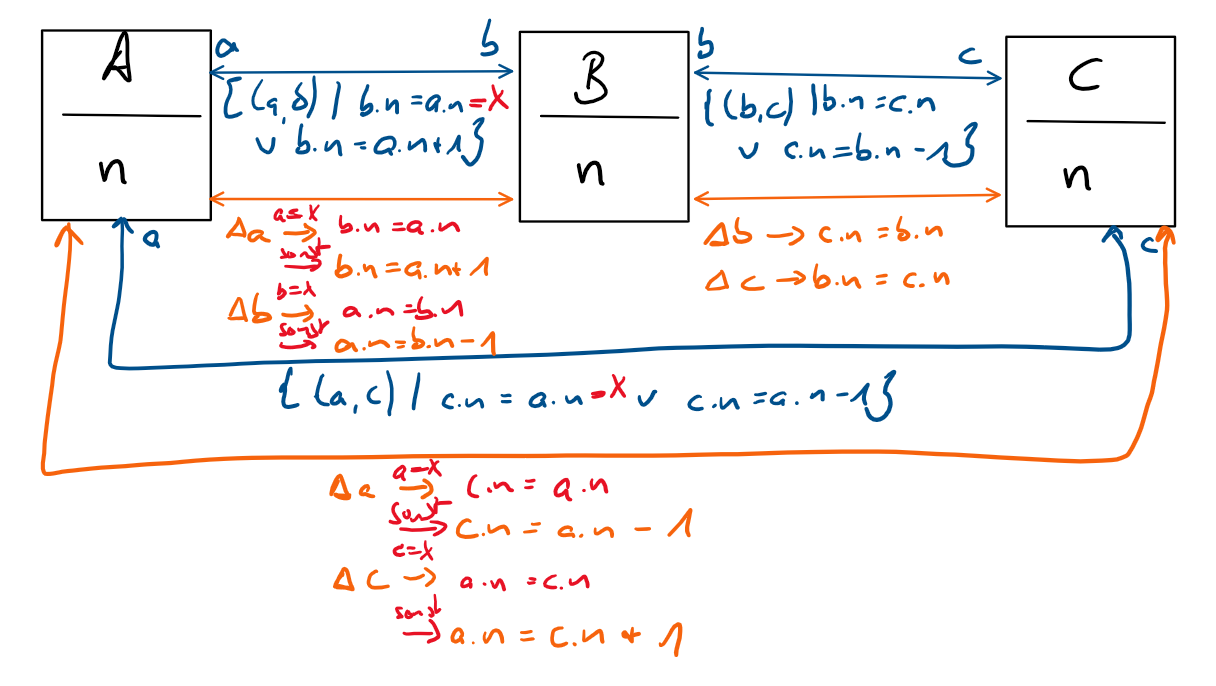
\includegraphics[width=\textwidth]{figures/correctness/formal/no_upper_bound_example.png}
    \caption{Example for no upper bound}
    \label{fig:formal:noupperboundexample}
\end{figure}

Depending on the value X, the transformations have to be executed X times to result in a consistent state. This value can be arbitrarily chosen, thus an arbitrary number of executions may be necessary to terminate in a consistent state.

From an engineering perspective, this is still unwanted behavior. We claim that a transformation network that takes thousands of executions of the same transformation to find a consistent state works not as expected and if running into a failure would expose severe problems to find the reasons for that failures.
Thus, we propose to simply abort the execution after some time to be sure not to run in an endless loop.

Finally, this problem is comparable to ordinary programming, because there the same situations regarding alternation and divergence can occur that result in non-termination of a program.
As we all know, it is impossible to systematically avoid that, but just possible to carefully develop the program and apply best practices to avoid such situations.

In the following, we propose measures to reduce the number of cases in which problematic cases can occur.
In a case study, we will see that using such measures already resolves most of the problems that can occur.
Additionally, we propose an orchestration strategy that improves the possibility to find errors in case something goes wrong.

\textbf{Central insight:} Alternation / Divergence cannot be avoided systematically (like in ordinary programming), if not restricting transformations in a way that may not be reasonable.

\subsection{Reducing Conservativeness of the Application Function}

Goal: Find a solution in as many cases as possible, abort in the others (conservatively). There are two approaches to achieve that: 
1. Reduce the number of cases in which there is no solution by adding assumptions to the relations and transformations (restrict input of app function)
2. Improve the ability to find a solution if it exists (improve capabilities of app function)
Secondary goal: In cases, in which no solution is found, support the user in understanding why no solution was found.


Regarding 1: Reduce problematic cases


1. reduce cases in which there is no such solution
1.1. On relation level: Only sets, so analysis possible.
Ensure that relations are defined in a way such that they do not allow a locally correct set of CPRs that has no APP solution. If there is a pair of models (or elements of a fine-grained relation) in a relation, a CPR may return it. But if there is no consistent tuple of models containing these two, it does not make any sense to consider these elements (even worse, if we have monotony, adding these elements makes the network unsolvable). For that reason, we need compatibility. Avoids both alternation and divergence
1.2. On transformation level: Hard to perform analyses
Require monotony to avoid alternation
Give some example why divergence cannot easily be avoided, thus terminate at some point
2. find the solution in as many cases as possible -> reasonable orchestration strategy
Focus on engineering solution 


Thus, there arise two questions:
- Although theoretically easy, how to practically define a CPR that is synchronizing?
- How to define an APP function and which requirements does that impose?




\section{Optimality rather than Correctness}

\mnote{Achieving a correct application function}
The definition of the application function basically ensures that the function either returns $\bot$ or executes the \modellevelconsistencypreservationrules given by the orchestration function to retrieve a changes tuple of models.
It is considered \emph{correct} if it ensures that its result is either $\bot$ or a consistent model tuple by executing the \modellevelconsistencypreservationrules given by the orchestration function.
% A correct application function thus has to ensure that its result is either $\bot$ or a consistent model tuple by executing the \modellevelconsistencypreservationrules given by the orchestration function.
In consequence, the application function can be realized by simply executing the result of the orchestration function and check whether the resulting model tuple is consistent or not and return an appropriate result.
Such a realization is generic and does not depend on the actual consistency preservation rules and orchestration function but represents a generic behavior.
Additionally, this gives an implementation of that function the ability to present a faulty result to the user, which eases finding out why no consistent state was reached.

\mnote{Correctness is not crucial}
Finally, correctness is not crucial, because correctness can easily be achieved by performing any execution of transformations and just ensuring that we terminate at some point in time and then decide whether the resulting models are consistent or not and appropriately deliver the result.

\mnote{How to define an orchestration function that is as optimal as possible?}
The remaining difficulty is how to define an orchestration function that fulfills the definition, i.e., to find a finite sequence of transformations, and also one that improves optimality, as an \emph{optimal} function can never be given.
Although the definition of the orchestration function proposes a closed description of that function, in practice such a function will not have a closed form but will be realized as an algorithm that dynamically decides which transformation to execute next.
Therefore the arising problem is that the length of the sequence to execute is not known a priori. Therefore, we need some abortion criterion. When a consistent result is found, this criterion is easy. But since we do not know whether a sequence exist, we need an abortion criterion that is reasonable and does not cut off the process although a consistent solution could be found, thus reducing optimality.
A simple realization for that algorithm to deliver a finite sequence of transformations would be to define a fixed termination criterion, such as a specific number of transformation executions. However, there is no upper bound for the number of executed transformations necessary to achieve consistency. Still, a fixed number (even 0) could be defined for the number of executed transformations to fulfill the definition. Hence, optimality would be 0 then as a consistent result is never reached. We therefore discuss in the following how to define an appropriate orchestration function and how to optimize it.

\mnote{Achieving a correct application function}
The definition of the application function basically ensures that the function either returns $\bot$ or executes the \modellevelconsistencypreservationrules given by the orchestration function to retrieve a changes tuple of models.
It is considered \emph{correct} if it ensures that its result is either $\bot$ or a consistent model tuple by executing the \modellevelconsistencypreservationrules given by the orchestration function.
% A correct application function thus has to ensure that its result is either $\bot$ or a consistent model tuple by executing the \modellevelconsistencypreservationrules given by the orchestration function.
In consequence, the application function can be realized by simply executing the result of the orchestration function and check whether the resulting model tuple is consistent or not and return an appropriate result.
Such a realization is generic and does not depend on the actual consistency preservation rules and orchestration function but represents a generic behavior.
Additionally, this gives an implementation of that function the ability to present a faulty result to the user, which eases finding out why no consistent state was reached.

\mnote{Correctness is not crucial}
Finally, correctness is not crucial, because correctness can easily be achieved by performing any execution of transformations and just ensuring that we terminate at some point in time and then decide whether the resulting models are consistent or not and appropriately deliver the result.

\mnote{How to define an orchestration function that is as optimal as possible?}
The remaining difficulty is how to define an orchestration function that fulfills the definition, i.e., to find a finite sequence of transformations, and also one that improves optimality, as an \emph{optimal} function can never be given.
Although the definition of the orchestration function proposes a closed description of that function, in practice such a function will not have a closed form but will be realized as an algorithm that dynamically decides which transformation to execute next.
Therefore the arising problem is that the length of the sequence to execute is not known a priori. Therefore, we need some abortion criterion. When a consistent result is found, this criterion is easy. But since we do not know whether a sequence exist, we need an abortion criterion that is reasonable and does not cut off the process although a consistent solution could be found, thus reducing optimality.
A simple realization for that algorithm to deliver a finite sequence of transformations would be to define a fixed termination criterion, such as a specific number of transformation executions. However, there is no upper bound for the number of executed transformations necessary to achieve consistency. Still, a fixed number (even 0) could be defined for the number of executed transformations to fulfill the definition. Hence, optimality would be 0 then as a consistent result is never reached. We therefore discuss in the following how to define an appropriate orchestration function and how to optimize it.

\textbf{Overall Goal:} Find correct orchestration function that improves optimality.

There are two ways to improve optimality of the orchestration function:
\begin{enumerate}
    \item Optimize the orchestration function, i.e., find a good order (probably this is not possible), at least find an order that helps the developer to find problems
    \item Optimize the input, i.e., define requirements to the transformations and their relations representing the input to optimize optimality
\end{enumerate}
\todo{We need an example for that}

Both goes hand in hand, because restrictions to the input can never lead to an orchestration function that always terminates without leading to unsupported relevant cases.

This conform to two approaches:
\begin{enumerate}
    \item Dynamic decision about selected transformation and abortion criteria
    \item Constructive restrictions that ensure that appropriate order is (easily) found
\end{enumerate}

\todo{Application function can be generically defined, orchestration maybe not? We actually want to ensure that both are generic and none of them has to be defined for a specific project.}


\begin{insight}[Orchestration]
    We have proven that orchestration of modular and independently developed transformations is undecidable without restrictions to the individual transformations.
    We found that there are no reasonable restrictions to the individual transformations that make orchestration decidable.
    In consequence, transformation orchestration needs to be conservative.
    In addition to reducing conservativeness, it can be useful to find an orchestration strategy that supports developers and users of transformation to find the reason for a transformation network not finding a consistent result after certain changes.
    One such strategy is given by inductively restoring consistency for subsets of the transformations and thus improving reasoning about provenance whenever consistency cannot be restored.
\end{insight}